\documentclass[border=20pt, tikz]{standalone}
\usepackage{tikz}
\usepackage{amsmath,amssymb}
\usetikzlibrary{positioning, arrows.meta, fit, backgrounds, calc, shapes.geometric}

% ==============================================================================
%  HYALINE V2-D: GLOBAL PIPELINE OVERVIEW
% ==============================================================================

% --- Colors ---
\definecolor{inputCol}{HTML}{1a1a2e}
\definecolor{preprocCol}{HTML}{16213e}
\definecolor{featureCol}{HTML}{0f3460}
\definecolor{modelCol}{HTML}{533483}
\definecolor{headCol}{HTML}{e94560}
\definecolor{outputCol}{HTML}{e94560}
\definecolor{boxBg}{HTML}{f8f9fa}

\begin{document}
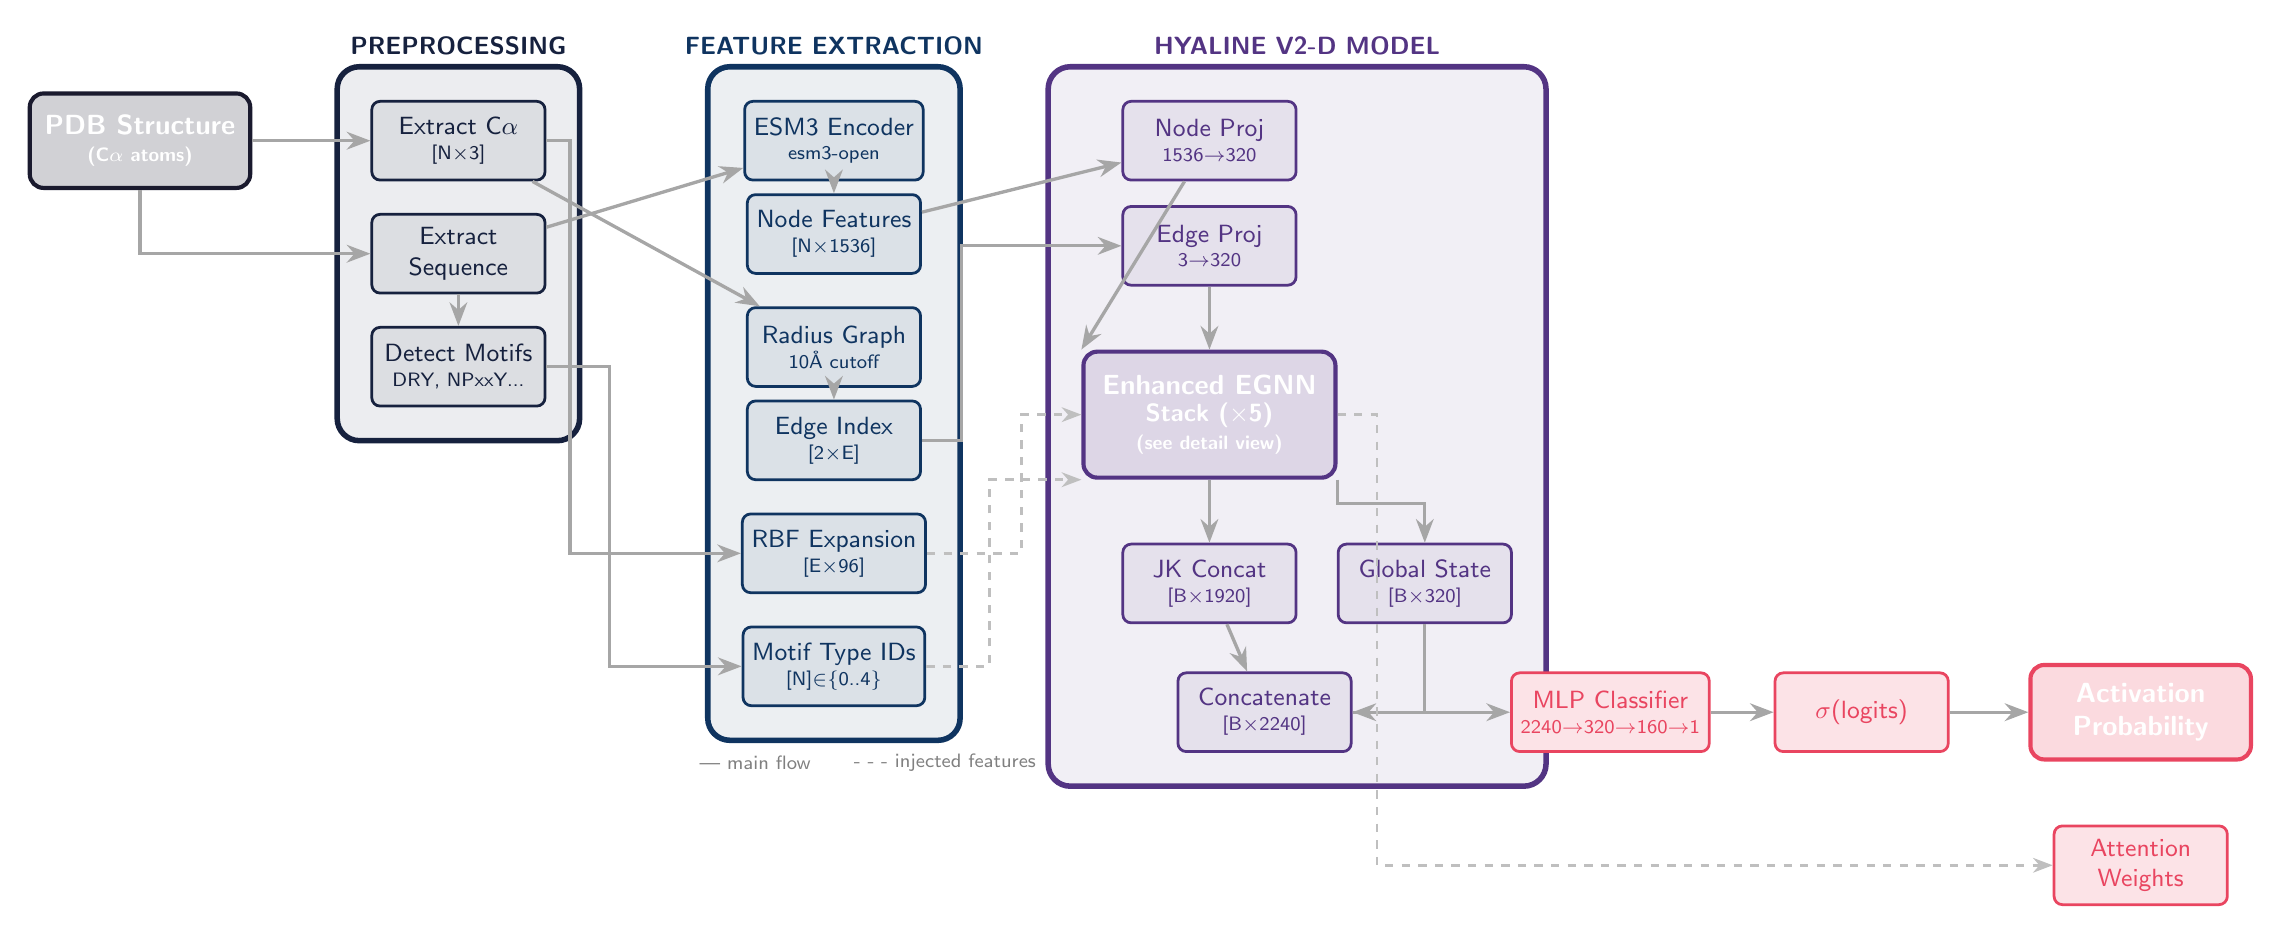
\begin{tikzpicture}[
    % Node styles
    block/.style={
        rectangle, 
        rounded corners=3pt,
        draw=#1, 
        fill=#1!15,
        text=#1,
        font=\sffamily\small,
        minimum height=1cm,
        minimum width=2.2cm,
        align=center,
        line width=1pt
    },
    bigblock/.style={
        rectangle,
        rounded corners=5pt,
        draw=#1,
        fill=#1!20,
        text=white,
        font=\sffamily\bfseries,
        minimum height=1.2cm,
        minimum width=2.8cm,
        align=center,
        line width=1.5pt
    },
    stage/.style={
        rectangle,
        rounded corners=8pt,
        draw=#1,
        line width=2pt,
        fill=#1!8,
        inner sep=12pt
    },
    stagelabel/.style={
        font=\sffamily\bfseries\small,
        text=#1
    },
    arrow/.style={
        ->,
        >={Stealth[length=3mm]},
        line width=1.2pt,
        draw=gray!70
    },
    dashedarrow/.style={
        ->,
        >={Stealth[length=2.5mm]},
        line width=1pt,
        draw=gray!50,
        dashed
    }
]

    % ==== INPUT STAGE ====
    \node[bigblock=inputCol] (pdb) {PDB Structure\\[-2pt]{\scriptsize(C$\alpha$ atoms)}};
    
    % ==== PREPROCESSING STAGE ====
    \node[block=preprocCol, right=1.5cm of pdb] (coords) {Extract C$\alpha$\\[-2pt]{\scriptsize[N$\times$3]}};
    \node[block=preprocCol, below=0.4cm of coords] (seq) {Extract\\Sequence};
    \node[block=preprocCol, below=0.4cm of seq] (motifdet) {Detect Motifs\\[-2pt]{\scriptsize DRY, NPxxY...}};
    
    % Preprocessing box
    \begin{scope}[on background layer]
        \node[stage=preprocCol, fit=(coords)(seq)(motifdet), label={[stagelabel=preprocCol]above:PREPROCESSING}] (prepbox) {};
    \end{scope}
    
    % ==== FEATURE EXTRACTION STAGE ====
    \node[block=featureCol, right=2.5cm of coords] (esm3) {ESM3 Encoder\\[-2pt]{\scriptsize esm3-open}};
    \node[block=featureCol, below=0.15cm of esm3] (emb) {Node Features\\[-2pt]{\scriptsize[N$\times$1536]}};
    
    \node[block=featureCol, below=0.4cm of emb] (graph) {Radius Graph\\[-2pt]{\scriptsize 10\AA\ cutoff}};
    \node[block=featureCol, below=0.15cm of graph] (edge) {Edge Index\\[-2pt]{\scriptsize[2$\times$E]}};
    
    \node[block=featureCol, below=0.4cm of edge] (rbf) {RBF Expansion\\[-2pt]{\scriptsize[E$\times$96]}};
    
    \node[block=featureCol, below=0.4cm of rbf] (motifemb) {Motif Type IDs\\[-2pt]{\scriptsize[N]$\in$\{0..4\}}};
    
    % Feature box
    \begin{scope}[on background layer]
        \node[stage=featureCol, fit=(esm3)(emb)(graph)(edge)(rbf)(motifemb), label={[stagelabel=featureCol]above:FEATURE EXTRACTION}] (featbox) {};
    \end{scope}
    
    % ==== MODEL STAGE ====
    \node[block=modelCol, right=2.5cm of esm3] (nodeproj) {Node Proj\\[-2pt]{\scriptsize 1536$\to$320}};
    \node[block=modelCol, below=0.3cm of nodeproj] (edgeproj) {Edge Proj\\[-2pt]{\scriptsize 3$\to$320}};
    
    \node[bigblock=modelCol, below=0.8cm of edgeproj, minimum width=3.2cm, minimum height=1.6cm] (egnn) {Enhanced EGNN\\[-2pt]{\small Stack ($\times$5)}\\[-2pt]{\scriptsize\textit{(see detail view)}}};
    
    \node[block=modelCol, below=0.8cm of egnn] (jk) {JK Concat\\[-2pt]{\scriptsize[B$\times$1920]}};
    \node[block=modelCol, right=0.5cm of jk] (globalst) {Global State\\[-2pt]{\scriptsize[B$\times$320]}};
    \node[block=modelCol, below=0.6cm of jk, xshift=0.7cm] (concat) {Concatenate\\[-2pt]{\scriptsize[B$\times$2240]}};
    
    % Model box
    \begin{scope}[on background layer]
        \node[stage=modelCol, fit=(nodeproj)(edgeproj)(egnn)(jk)(globalst)(concat), label={[stagelabel=modelCol]above:HYALINE V2-D MODEL}] (modelbox) {};
    \end{scope}
    
    % ==== HEAD & OUTPUT STAGE ====
    \node[block=headCol, right=2cm of concat] (mlp) {MLP Classifier\\[-2pt]{\scriptsize 2240$\to$320$\to$160$\to$1}};
    \node[block=headCol, right=0.8cm of mlp] (sigmoid) {$\sigma$(logits)};
    
    \node[bigblock=outputCol, right=1cm of sigmoid] (prob) {Activation\\Probability};
    \node[block=outputCol, below=0.8cm of prob] (attnw) {Attention\\Weights};
    
    % ==== CONNECTIONS ====
    
    % Input -> Preprocessing
    \draw[arrow] (pdb) -- (coords);
    \draw[arrow] (pdb) |- (seq);
    
    % Preprocessing internal
    \draw[arrow] (seq) -- (motifdet);
    
    % Preprocessing -> Features
    \draw[arrow] (coords) -- (graph);
    \draw[arrow] (coords.east) -- ++(0.3,0) |- (rbf.west);
    \draw[arrow] (seq) -- (esm3);
    \draw[arrow] (motifdet.east) -- ++(0.8,0) |- (motifemb.west);
    
    % Features internal
    \draw[arrow] (esm3) -- (emb);
    \draw[arrow] (graph) -- (edge);
    
    % Features -> Model
    \draw[arrow] (emb) -- (nodeproj);
    \draw[arrow] (edge.east) -- ++(0.5,0) |- (edgeproj.west);
    
    % Model internal
    \draw[arrow] (nodeproj) -- (egnn.north west);
    \draw[arrow] (edgeproj) -- (egnn.north);
    \draw[dashedarrow] (rbf.east) -- ++(1.2,0) |- (egnn.west);
    \draw[dashedarrow] (motifemb.east) -- ++(0.8,0) |- (egnn.south west);
    
    \draw[arrow] (egnn) -- (jk);
    \draw[arrow] (egnn.south east) -- ++(0,-.3) -| (globalst.north);
    \draw[arrow] (jk) -- (concat);
    \draw[arrow] (globalst) |- (concat);
    
    % Model -> Head -> Output
    \draw[arrow] (concat) -- (mlp);
    \draw[arrow] (mlp) -- (sigmoid);
    \draw[arrow] (sigmoid) -- (prob);
    
    % Attention output branch
    \draw[dashedarrow] (egnn.east) -- ++(0.5,0) |- (attnw.west);
    
    % ==== LEGEND ====
    \node[below=0.5cm of motifemb, xshift=-1cm, font=\sffamily\scriptsize, text=gray] (leg1) {--- main flow};
    \node[right=0.3cm of leg1, font=\sffamily\scriptsize, text=gray] {- - - injected features};

\end{tikzpicture}
\end{document}